\capitulo{5}{Resultados}

En este capítulo se presentan los resultados obtenidos tras la implementación y evaluación de diferentes arquitecturas de segmentación aplicadas a las estructuras del cerebelo fetal, con el objetivo de analizar y comparar su rendimiento.

\section{Resumen de resultados.}
Durante el desarrollo experimental del proyecto se ha llevado a cabo la implementación de un sistema de segmentación basado en la biblioteca \texttt{segmentation\_models.pytorch}. Se partió de un conjunto de imágenes de ecografías 2D del cerebro fetal en un plano transcerebeloso, proporcionadas por el Servicio de Ginecología del HUBU. 

A partir de estas imágenes se generaron sus máscaras \textit{ground truth}, en las que se anotaron las estructuras anatómicas del cerebelo de interés. Estas máscaras, junto con las imágenes originales, conformaron el conjunto de datos empleado para el entrenamiento de las distintas arquitecturas basadas en redes neuronales convolucionales (CNN). Finalmente, se calcularon diversas métricas de rendimiento que permitieron analizar y comparar el desempeño de cada una de las arquitecturas evaluadas. 

A continuación, se presentan y analizan los resultados obtenidos, comparando diferentes arquitecturas y parámetros, lo cual ha permitido fundamentar la elección del modelo final.

\subsection{Arquitecturas}
\subsubsection{U-Net}
Es una arquitectura tipo \textit{encoder-decoder}, que mediante el uso de abundantes conexiones de salto (\textit{skip connections}), permite combinar el contexto global capturado durante la compresión con los detalles espaciales recuperados en la fase de expansión. Esta integración mejora significativamente la precisión en tareas de segmentación biomédica, al conservar tanto la información contextual como la resolución espacial \cite{unet2015}.
\subsubsection{U-Net++}
\texttt{U-Net++} es una variante de \texttt{U-Net} que introduce una estructura de conectividad más densa entre el codificador y el decodificador. A través de una serie de subdecodificadores intermedios, esta arquitectura refina progresivamente los mapas de características a diferentes profundidades, lo que optimiza la fusión semántica entre escalas y reduce la discrepancia entre las representaciones generadas por el encoder y el decoder \cite{unetplusplus2018}.
\subsubsection{MAnet}
Presenta una arquitectura encoder-decoder similar a \texttt{U-Net}, pero incorpora un módulo de atención múltiple. Este mecanismo permite a la red reforzar dinámicamente la importancia de distintas regiones espaciales y canales de características durante el proceso de reconstrucción. La aplicación jerárquica de esta atención mejora la extracción de características discriminativas, dando como resultado una segmentación más precisa y robusta \cite{manet2020}.
\subsubsection{Linknet}
\texttt{LinkNet} se distingue por la implementación de conexiones directas (\textit{skip connections}) entre los bloques del codificador y sus correspondientes en el decodificador. Estas conexiones permiten reutilizar características previamente extraídas, lo que optimiza la reconstrucción espacial de la imagen y reduce la pérdida de información durante la etapa de codificación \cite{linknet2020}. Como resultado, se obtiene una segmentación eficiente con menor consumo computacional.
\subsubsection{FPN}
La \texttt{FPN} (Feature Pyramid Network) utiliza una estructura piramidal para la fusión de mapas de características a distintas escalas. Mediante una ruta de arriba hacia abajo y conexiones laterales, esta arquitectura mejora la detección y segmentación de objetos de diferentes tamaños \cite{fpnpresentation}.

\begin{figure}[h]
    \centering
    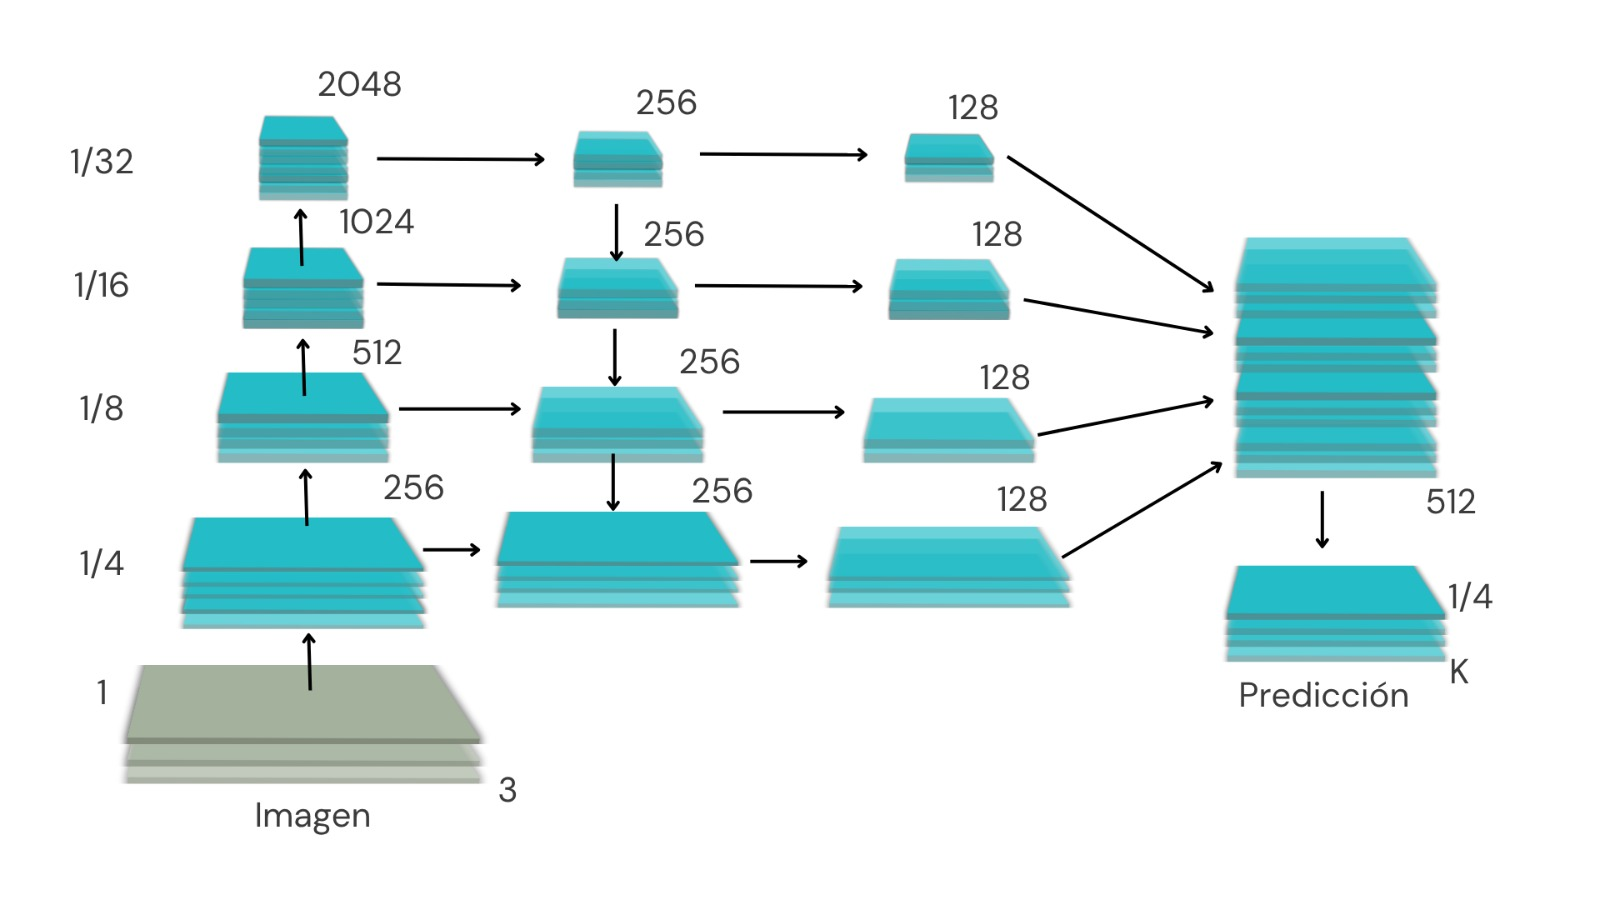
\includegraphics[width= \textwidth]{img/fpn_estructura.jpeg}
    \caption{Esquema de una arquitectura tipo FPN para segmentación semántica. Figura original basada en \cite{fpnpresentation} }
    \label{fig:fpn_diagrama}
\end{figure}

\subsubsection{PSPNet} 
Esta arquitectura introduce un módulo de agrupación piramidal (\textit{pyramid pooling module}), diseñado para capturar información contextual global a múltiples escalas. Este módulo realiza agrupaciones espaciales con diferentes tamaños de ventana sobre el mapa de características, lo que permite a la red integrar tanto contexto global como detalles locales. Gracias a este enfoque, \texttt{PSPNet} es útil en escenarios complejos donde la variabilidad de objetos dificulta una segmentación precisa \cite{pspnet2017}.

Todas las arquitecturas anteriores utilizan el modelo \texttt{resnext50\_32x4d} \footnote{Documentación de resnext50\_32x4d: \url{https://docs.pytorch.org/vision/main/models/generated/torchvision.models.resnext50_32x4d.html}} como encoder preentrenado en \texttt{ImageNet}. Esta arquitectura se basa en el diseño de \texttt{ResNeXt}, incorporando 32 grupos de convoluciones con una anchura de 4. Esto permite mejorar la capacidad de extracción de características sin incrementar significativamente el número de parámetros, lo que hace que sea una opción eficiente para tareas de segmentación.

Para evaluar el rendimiento de estas arquitecturas, se ha realizado un análisis sobre un conjunto de test compuesto por cuatro imágenes. En la Tabla \ref{tab:resultados_sindataaumentation} se presentan los valores medios de precisión e \texttt{IoU} obtenidos en cada arquitectura, destacando la importancia del \texttt{IoU} como métrica fundamental en tareas de segmentación.

\begin{table}[h]
    \centering
    \begin{tabular}{lcc}
    \textbf{Arquitectura} & \textbf{Precisión media (\%)} & \textbf{IoU media (\%)} \\
    \hline
    U-Net             & 49,13 & 45,27\\
    U-Net++           & 49,05 & 45,34\\
    FPN               & 54,08 & 49,88\\
    PSPNet            & 16,56 & 14,75\\
    LinkNet           & 64.05 & 56,83\\
    MAnet             & 55,56 & 43,72\\
    \hfill
    \end{tabular}
    \caption{Comparativa de métricas medias por arquitectura sobre el conjunto de test.} \label{tab:resultados_sindataaumentation}
\end{table}

Con el objetivo de evaluar la robustez del modelo ante variaciones en los datos de entrada, se ha aplicado \textit{data augmentation} sobre el conjunto de test. Las transformaciones utilizadas incluyen rotaciones aleatorias, cambios de escala y ajuste de contraste, con el fin de simular condiciones diversas y mejorar la capacidad de generalización del modelo. La Tabla \ref{tab:resultados_condataaumentation} presenta los resultados obtenidos tras la aplicación de estas técnicas, permitiendo comparar su impacto en la precisión y el \texttt{IoU}.

\begin{table}[h]
    \centering
    \begin{tabular}{lcc}
    \textbf{Arquitectura} & \textbf{Precisión media (\%)} & \textbf{IoU media (\%)} \\
    \hline
    U-Net             & 71,91 & 62,15\\
    U-Net++           & 56,03 & 50,25\\
    FPN               & 59,76 & 54,99\\
    PSPNet            & 17 & 16,53\\
    LinkNet           & 51,77 & 48,22\\
    MAnet             & 56,78 & 35,30\\
    \hfill
    \end{tabular}
    \caption{Comparativa de métricas medias por arquitectura sobre el conjunto de test con data augmentation.} \label{tab:resultados_condataaumentation}
\end{table}

 Tras comparar los resultados obtenidos con y sin \textit{data augmentation}, se observa una mejora generalizada en la mayoría de las arquitecturas, especialmente en la métrica \texttt{IoU}, que resulta la más relevante para la tarea de segmentación. Por tanto, se ha decidido conservar las configuraciones con \textit{data augmentation} como base para la evaluación final.

 Por otro lado, el análisis de las curvas de pérdida durante el entrenamiento reveló indicios de sobreajuste en las arquitecturas, donde la pérdida de validación deja de mejorar o incluso comienza a aumentar tras cierto número de épocas. 

\begin{figure}[h]
    \centering
    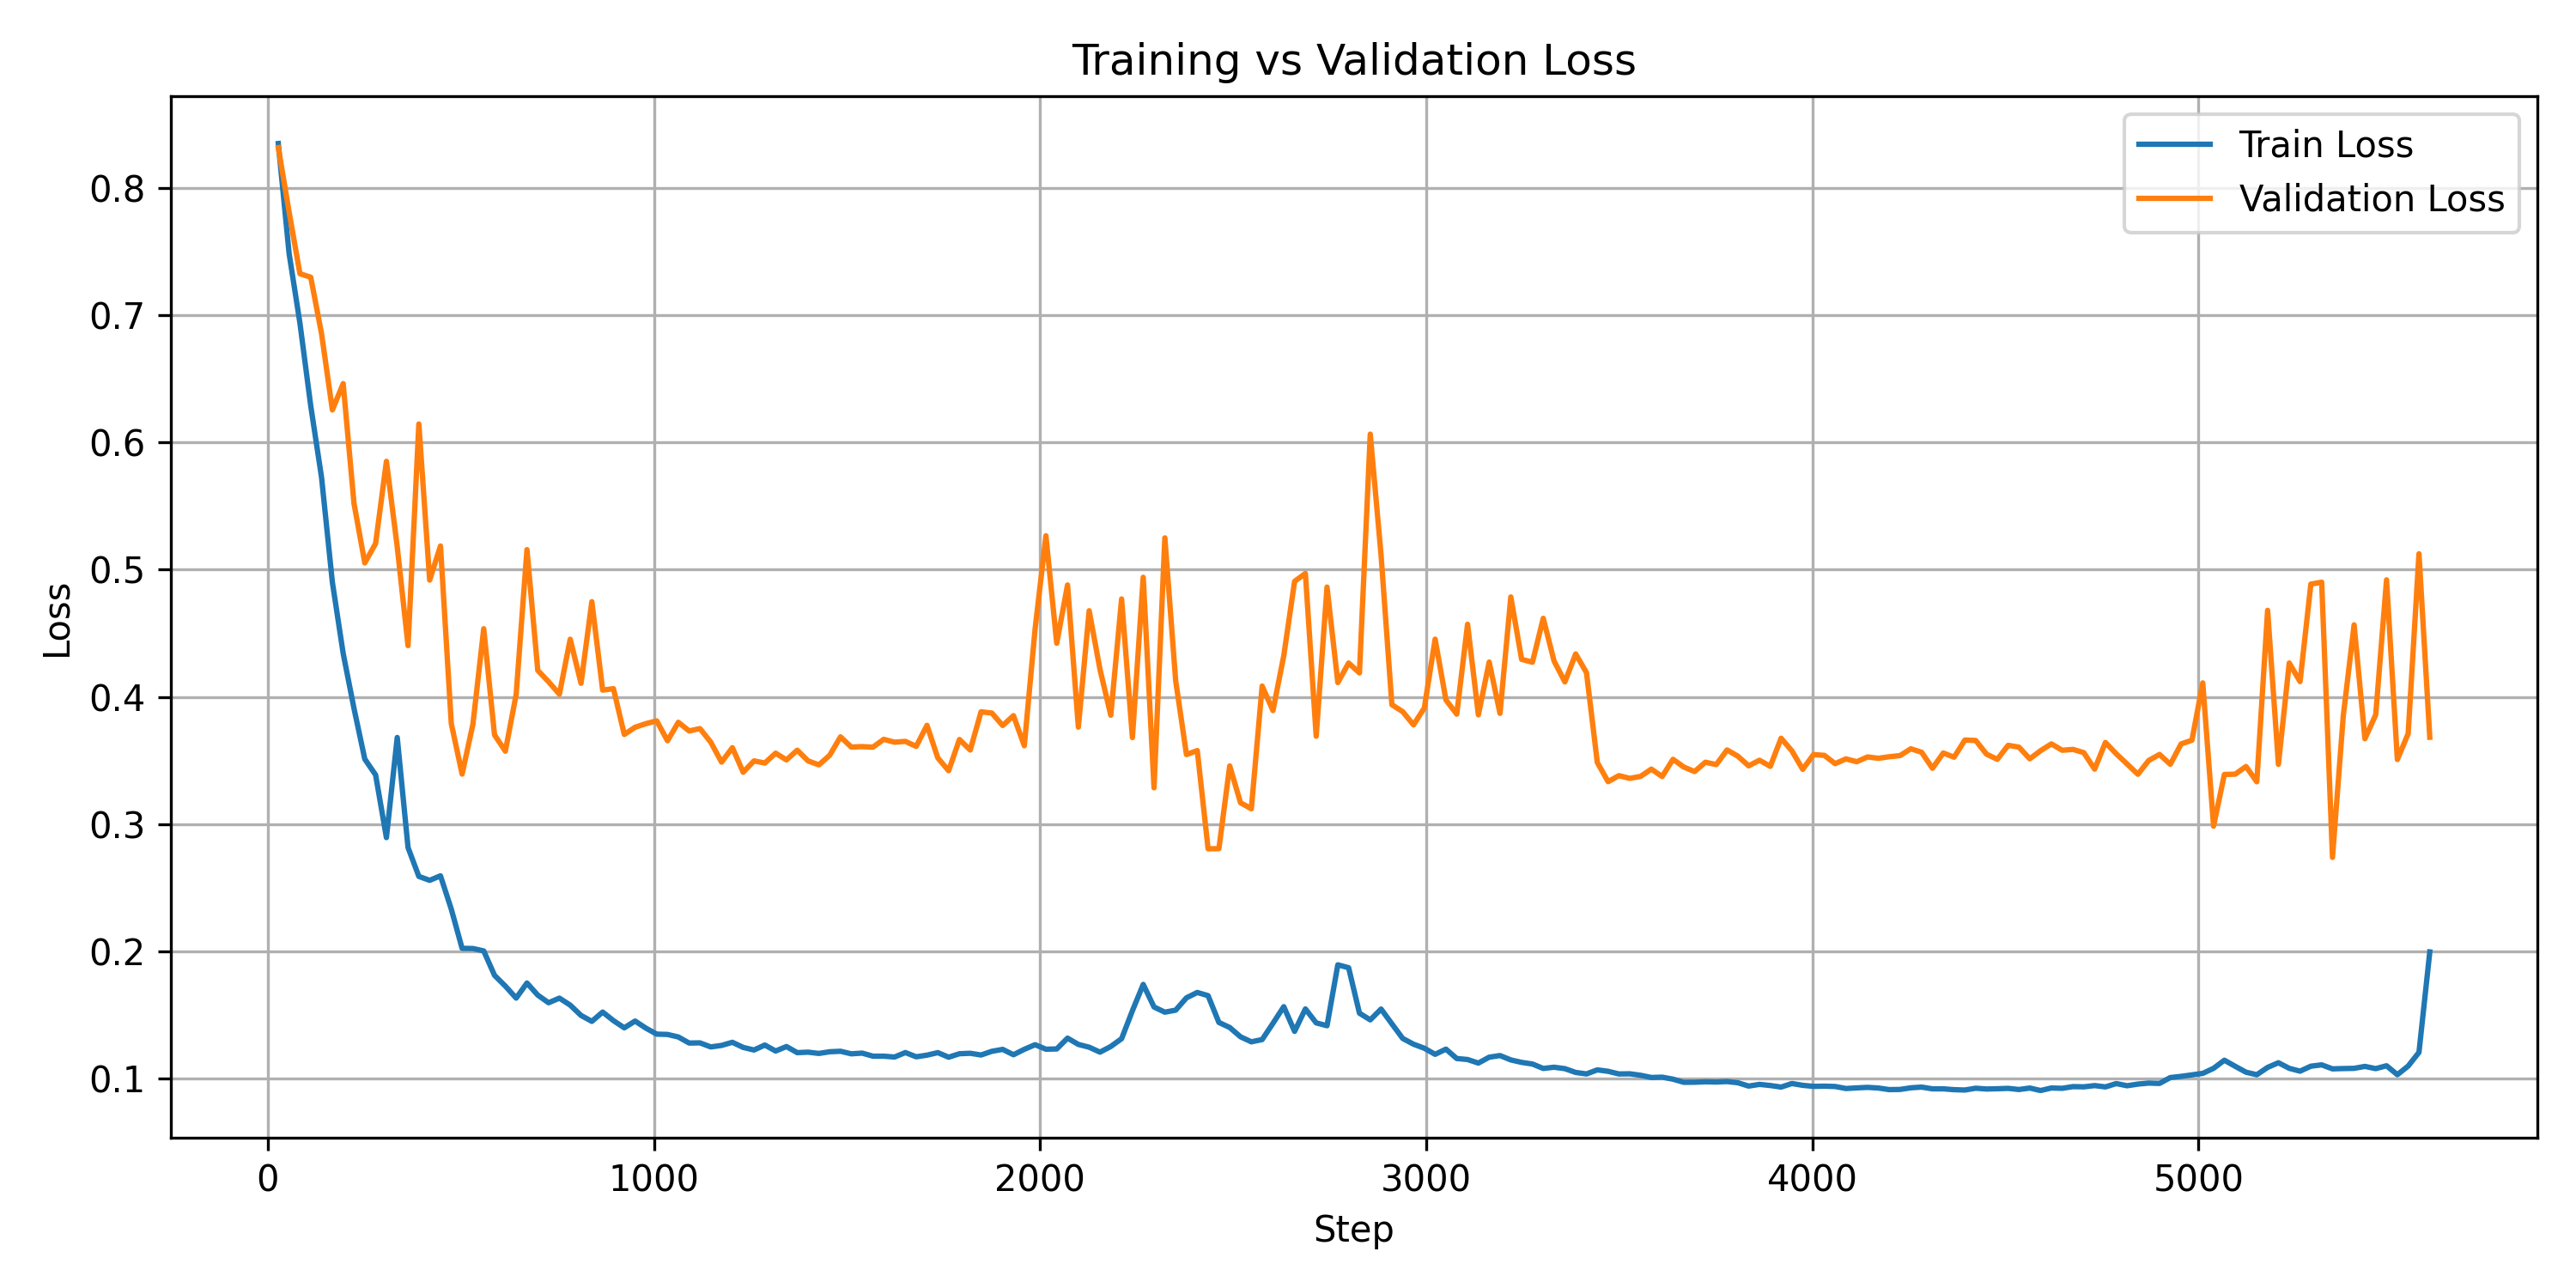
\includegraphics[width= \textwidth]{img/training_vs_validation_loss_manet.png}
    \caption{Curvas de pérdida: MAnet.}
    \label{fig:loss_manet}
\end{figure}

\begin{figure}[h]
    \centering
    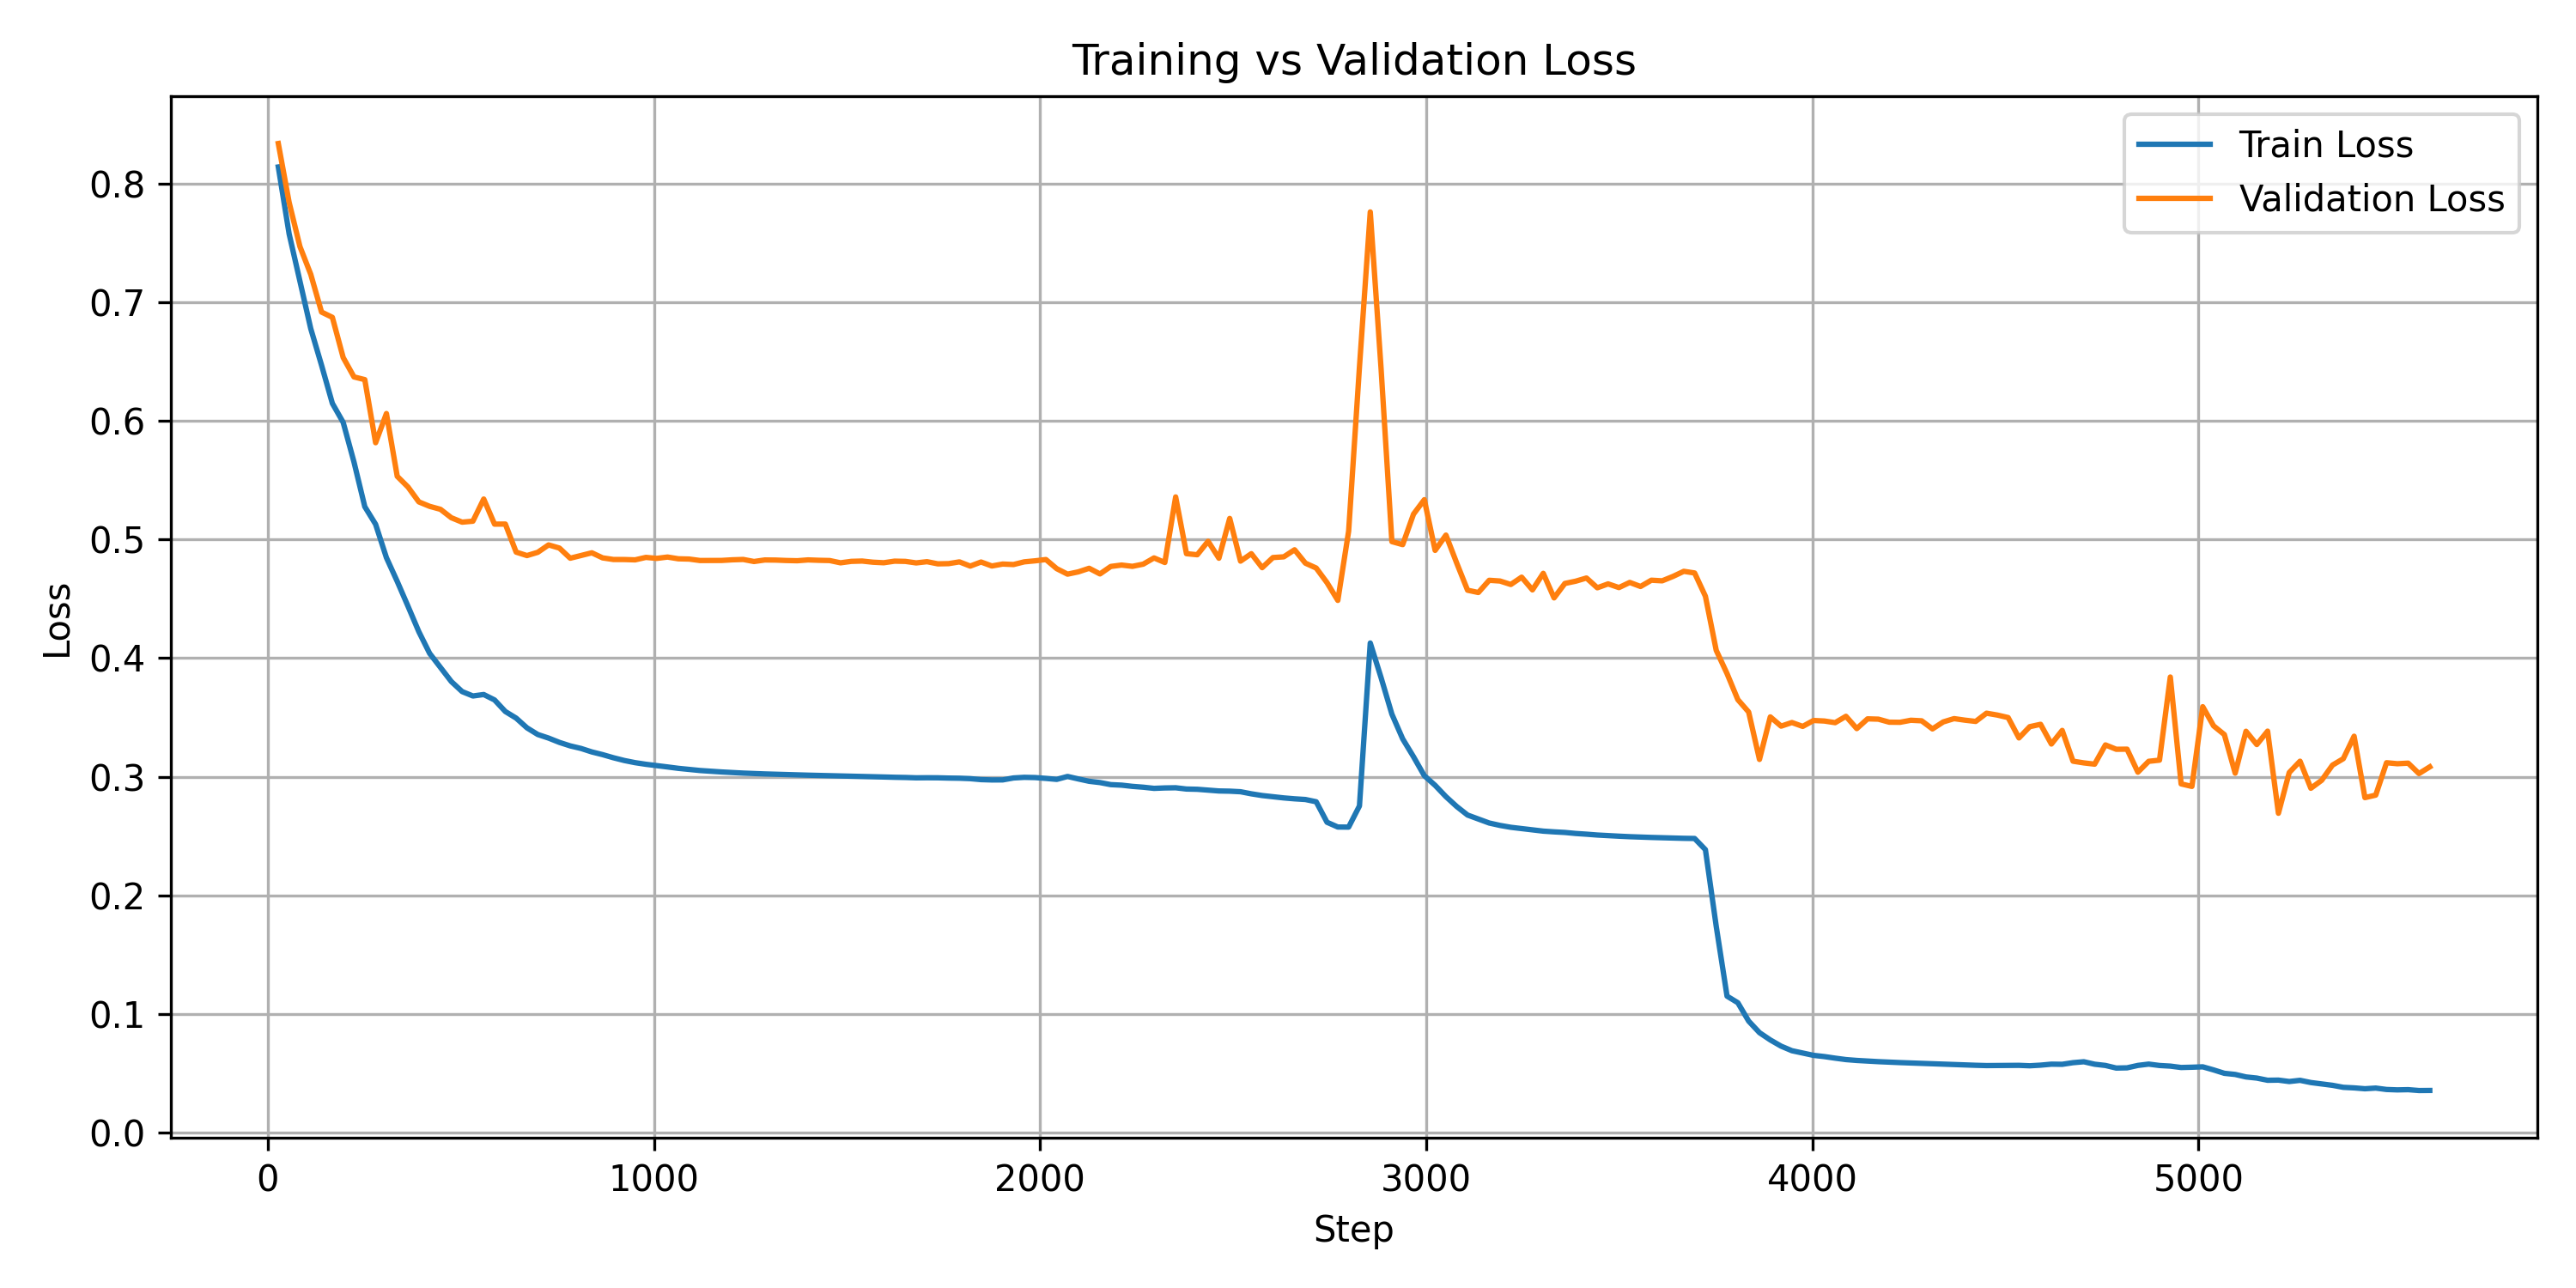
\includegraphics[width= \textwidth]{img/training_vs_validation_loss_unet.png}
    \caption{Curvas de pérdida: U-Net.}
    \label{fig:loss_unet}
\end{figure}

Como se observa en las Figuras \ref{fig:loss_manet} y \ref{fig:loss_unet}, la pérdida de entrenamiento disminuye de forma sostenida, mientras que la de validación tiende a estabilizarse o incluso incrementarse, lo que evidencia el inicio del sobreajuste y justifica la aplicación del criterio de parada anticipada.

Ante esta situación, se incorporó la técnica de \textit{early stopping} como mecanismo de regularización, configurada con una paciencia de 30 épocas sobre la métrica de validación.

\begin{figure}[h]
    \centering
    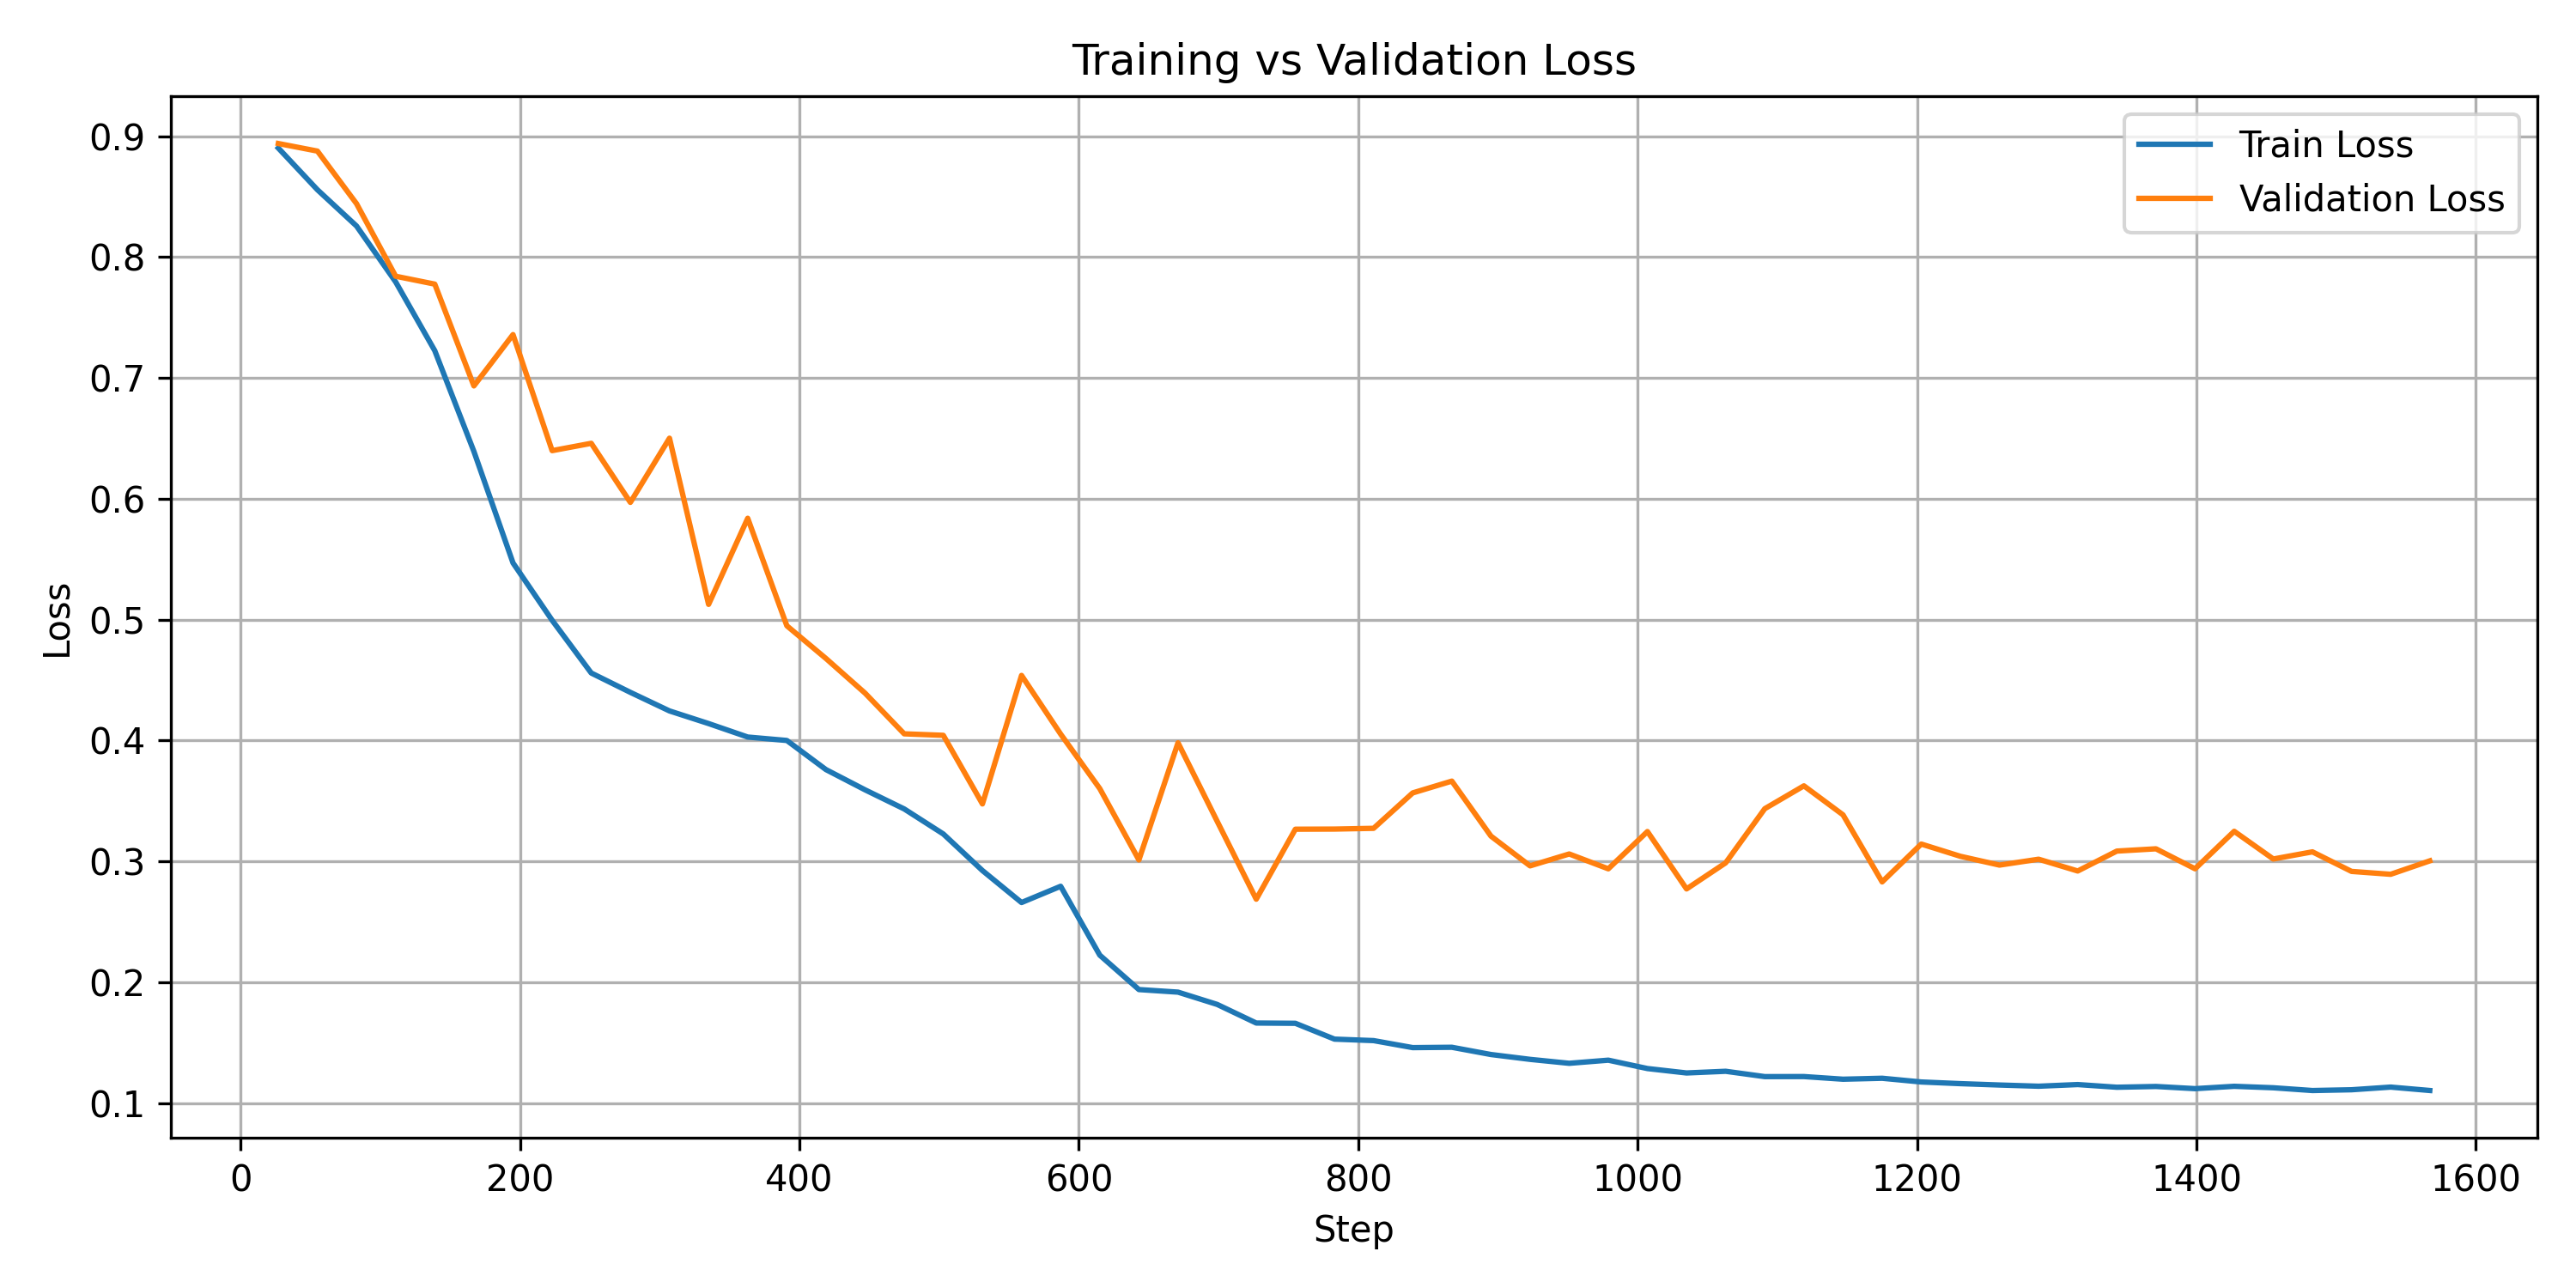
\includegraphics[width=1.1\textwidth]{img/training_vs_validation_loss.png}
    \caption{Curva de pérdida tras aplicar early stopping: U-Net.}
    \label{fig:loss_unet_earlystopping}
\end{figure}

La Figura \ref{fig:loss_unet_earlystopping} muestra un comportamiento específico del entrenamiento de U-Net con \textit{early stopping} activado. Se aprecia cómo el entrenamiento se interrumpe automáticamente al no observarse mejoras sustanciales en la pérdida de validación, lo que contribuye a una mayor eficiencia y generalización del modelo.

En la Tabla \ref{tab:resultados_earlystopping} se muestran los resultados cuantitativos obtenidos en el conjunto de test para cada arquitectura, una vez aplicada la estrategia de regularización.

\begin{table}[h]
    \centering
    \begin{tabular}{lcc}
    \textbf{Arquitectura} & \textbf{Precisión media (\%)} & \textbf{IoU media (\%)} \\
    \hline
    U-Net             & 70.74 & 63,69\\
    U-Net++           & 67,07 & 62,46\\
    FPN               & 70,77 & 60,23\\
    PSPNet            & 15,06 & 12,11\\
    LinkNet           & 71,12 & 60,32\\
    MAnet             & 61,49 & 55,62\\
    \hfill
    \end{tabular}
    \caption{Comparativa de métricas medias por arquitectura sobre el conjunto de test con early stopping.} \label{tab:resultados_earlystopping}
\end{table}

Los resultados muestran un rendimiento competitivo en la mayoría de arquitecturas, destacando LinkNet y FPN en precisión media, mientras que U-Net obtiene la mejor puntuación en \texttt{IoU}. En contraste, PSPNet presenta un rendimiento significativamente inferior, posiblemente debido a una menor capacidad de adaptación al dominio específico del conjunto de datos.

Finalmente, en la Figura \ref{fig:resultado_unet} se muestra un ejemplo representativo de segmentación realizado por U-Net sobre una imagen del conjunto de test. Se puede apreciar una segmentación precisa de las estructuras cerebrales, lo que confirma su capacidad de generalización bajo las condiciones de entrenamiento adoptadas.


\begin{figure}[h]
    \centering
    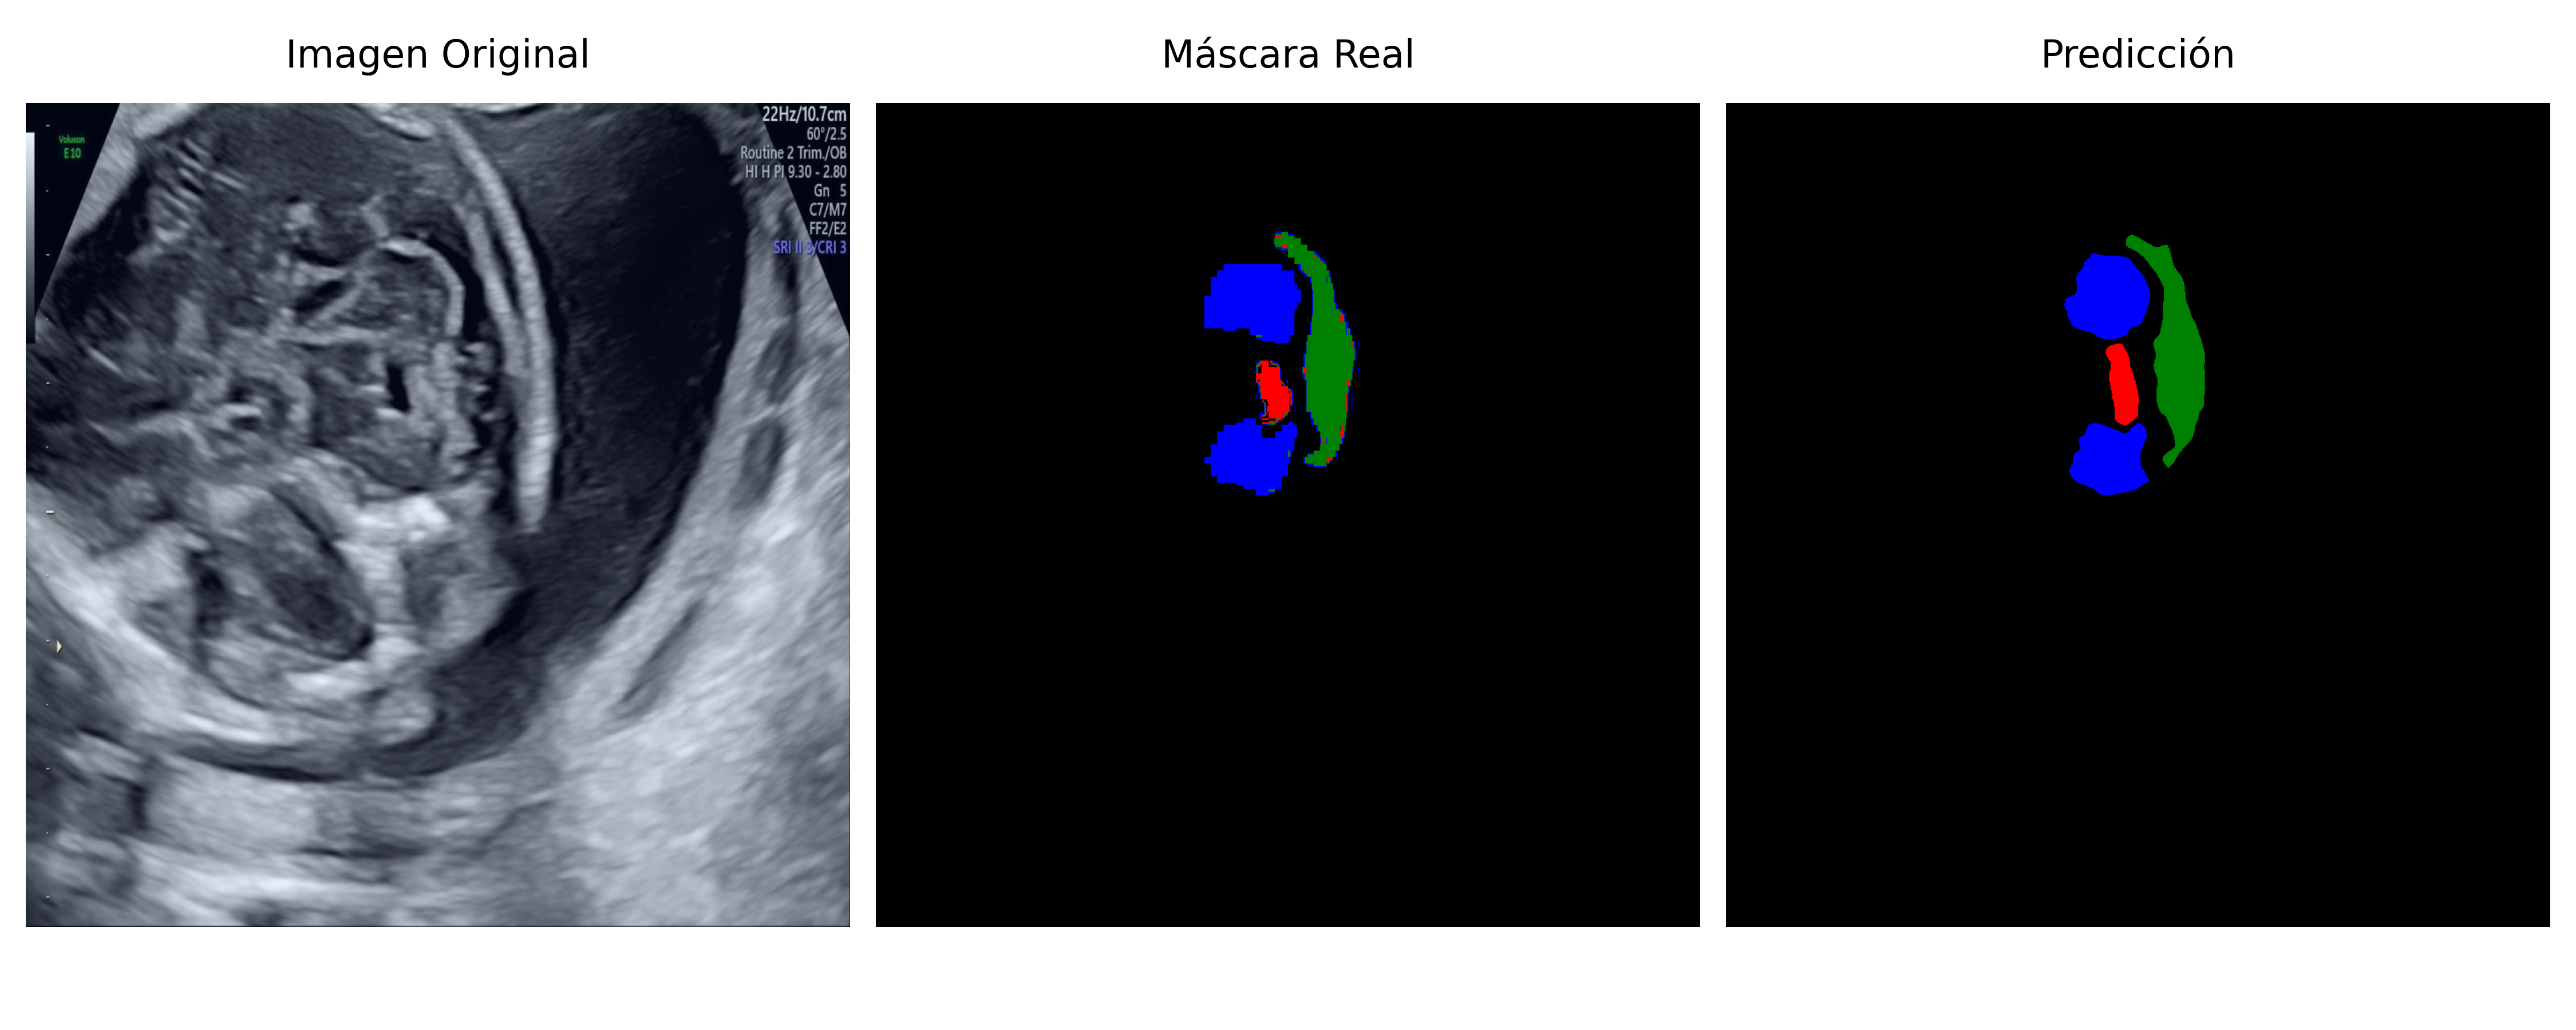
\includegraphics[width=1.1\textwidth]{img/image1_unet.png}
    \caption{Ejemplo de resultado con U-Net. Muestra la imagen original, el resultado de la predicción y la imagen ground truth.}
    \label{fig:resultado_unet}
\end{figure}
 
\section{Discusión.}

Los resultados obtenidos muestran un rendimiento sólido por parte de las arquitecturas evaluadas, destacando especialmente \texttt{U-Net}, que ha alcanzado la mayor puntuación en la métrica \texttt{IoU}. Dado que esta métrica refleja con mayor fidelidad la superposición entre la predicción y la verdad de terreno, se confirma la capacidad del modelo para identificar con precisión las estructuras anatómicas de interés, lo que la posiciona como la opción más adecuada para esta tarea.

La aplicación de \textit{data augmentation} ha demostrado ser una estrategia eficaz para mejorar la generalización. Su incorporación ha derivado en una mejora consistente en las métricas, especialmente en \texttt{IoU}, lo que sugiere que ha compensado adecuadamente la limitada variabilidad presente en el conjunto de datos original. Este resultado refuerza la importancia de emplear técnicas de aumento de datos en escenarios con restricciones muestrales.

Asimismo, la implementación de \textit{early stopping} con una paciencia de 30 épocas ha sido clave para prevenir el sobreajuste. Las curvas de pérdida analizadas evidencian que, sin este mecanismo, la pérdida de validación tiende a estabilizarse o incluso aumentar tras cierto número de épocas, mientras la pérdida de entrenamiento sigue disminuyendo. Este comportamiento es indicativo de un ajuste excesivo al conjunto de entrenamiento, especialmente en arquitecturas más complejas. La incorporación de \textit{early stopping} ha permitido detener el entrenamiento de forma óptima, reduciendo el riesgo de sobreajuste y mejorando la eficiencia computacional.

Respecto al desempeño específico de cada arquitectura, destaca el bajo rendimiento de \texttt{PSPNet}. A pesar de sus buenos resultados en otros dominios, su adaptación al presente escenario ha sido limitada, probablemente por factores como la resolución de las imágenes, el tipo de estructuras o la escasez relativa de los datos. En contraste, modelos como \texttt{LinkNet} y \texttt{FPN} han demostrado un equilibrio entre precisión y capacidad de generalización, posicionándose como alternativas sólidas a \texttt{U-Net}.

Finalmente, los ejemplos cualitativos analizados refuerzan los resultados cuantitativos, mostrando segmentaciones precisas de las principales estructuras cerebrales. Esto confirma que el modelo seleccionado es capaz de extraer representaciones relevantes incluso en un entorno clínico con alta variabilidad anatómica, lo que valida su aplicabilidad práctica. La estabilidad y precisión observada suponen un avance en la automatización del análisis anatómico y abren la puerta a futuras implementaciones en entornos reales de diagnóstico.